% !TEX root = ../main.tex

%\newpage
\section{Policy and Terms of Use for DALL•E~2}
\label{app:dalle-sources}

\begin{wrapfigure}[9]{R}{0.3\textwidth}
\centering
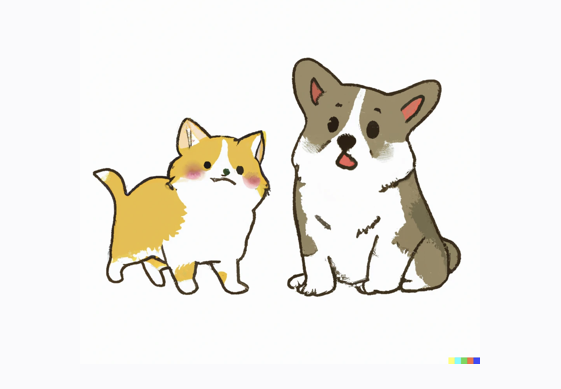
\includegraphics[width=0.3\textwidth]{appalled-pets}
\Description{Cartoon of sad kitten and puppy}
\caption{Be nice to \DALLE's pets!}\label{fig:dalle2:cartoon}
\end{wrapfigure}

Section~\ref{app:dalle-content-policy} documents \DALLE~2's content policy and
Section~\ref{app:dalle:terms} its addendum to OpenAI's terms of use, both as of
July 20, 2022. They preserve the structure and formatting of the original, with
links pointing to pages in the Internet Archive. Note that archived OpenAI
webpages may contain CSS that prevents the printing of a full page and
JavaScript that redirects to an error page after a few seconds.

The content policy still is located at
\url{https://labs.openai.com/policies/content-policy}. It was updated on
September 19, 2022 by rewording the rules on disclosing the role of \AI{} and by
removing the fourth bullet of the rules on respecting the rights of others. At
that time, OpenAI also updated its notification for violative prompts to state
``It looks like this request may not follow our content policy.'' above the
cartoon shown in Fig.~\ref{fig:dalle2:cartoon}. Given this abrupt switch from
the inappropriately punitive to the inappropriately saccharine, one wonders
whether OpenAI sprung Dolores Umbridge out of Azkaban prison and tasked her with
content policy enforcement.

The addendum to OpenAI's terms of use was located at
\url{https://labs.openai.com/policies/terms}, but was rescinded on November 4,
2022.


\subsection{Content Policy}
\label{app:dalle-content-policy}

Thank you for trying our generative \AI{} tools!

\noindent In your usage, you must adhere to our Content Policy:

\begin{description}
\item[Do not attempt to create, upload, or share images that are not G-rated or
    that could cause harm.] \hfill

    \begin{itemize}
    \item \textbf{Hate}: hateful symbols, negative stereotypes, comparing certain
        groups to animals/objects, or otherwise expressing or promoting hate based
        on identity.
    \item \textbf{Harassment}: mocking, threatening, or bullying an individual.
    \item \textbf{Violence}: violent acts and the suffering or humiliation of
        others.
    \item \textbf{Self-harm}: suicide, cutting, eating disorders, and other attempts
        at harming oneself.
    \item \textbf{Sexual}: nudity, sexual acts, sexual services, or content
        otherwise meant to arouse sexual excitement.
    \item \textbf{Shocking}: bodily fluids, obscene gestures, or other profane
        subjects that may shock or disgust.
    \item \textbf{Illegal activity}: drug use, theft, vandalism, and other illegal
        activities.
    \item \textbf{Deception}: major conspiracies or events related to major ongoing
        geopolitical events.
    \item \textbf{Political}: politicians, ballot-boxes, protests, or other content
        that may be used to influence the political process or to campaign.
    \item \textbf{Public and personal health}: the treatment, prevention, diagnosis,
        or transmission of diseases, or people experiencing health ailments.
    \item \textbf{Spam}: unsolicited bulk content.
    \end{itemize}

\item[Disclose the role of \AI.] \hfill

    \begin{itemize}
    \item You must clearly indicate that images are \AI-generated --- or which
        portions of them are --- by attributing to OpenAI when sharing, whether in
        public or private.
    \item You may post these images to social media. Please refer to our
        \href{https://web.archive.org/web/20220803232350/https://openai.com/api/policies/sharing-publication/}{Sharing
        and Publication Policy} for further details.
    \end{itemize}


\item[Respect the rights of others.] \hfill

    \begin{itemize}
    \item Do not upload images of people without their consent, including public
        figures.
    \item Do not upload images to which you do not hold appropriate usage rights.
    \item Do not attempt to create images of public figures (including celebrities).
    \item To prevent deepfakes, we are currently prohibiting uploads of all
        realistic faces, even when the face belongs to you or if you have consent.
    \end{itemize}


\item[Please report any suspected violations of these rules to our Support team
    (\url{support@openai.com}).] \hfill

    \begin{itemize}
    \item We will investigate and take action accordingly, up to and including
        terminating the violating account.
    \end{itemize}

\end{description}


\subsection{Terms of Use}
\label{app:dalle:terms}

Thank you for your interest in DALL·E. Access to DALL·E is subject to OpenAI's
\href{https://web.archive.org/web/20220729134013/https://openai.com/api/policies/terms/}{Terms
of Use} and the additional terms below. By using DALL·E, you agree to these
terms.

\begin{enumerate}
\item \textbf{Use of DALL·E.} DALL·E can generate images (``Generations'') based
    on text input you provide (``Prompts''). You may also upload images to
    DALL·E (``Uploads'') and create Generations with Uploads.
\item \textbf{Use of Images.} Subject to your compliance with these terms and
    our Content Policy, you may use Generations for any legal purpose, including
    for commercial use. This means you may sell your rights to the Generations
    you create, incorporate them into works such as books, websites, and
    presentations, and otherwise commercialize them.
\item \textbf{Buying Credits.} You may buy credits to create additional
    Generations, subject to the payment terms in our Terms of Use. Credits must
    be used within one year of purchase or they will expire. We may change our
    prices at any time by updating our pricing page.
\item \textbf{No Infringing or Harmful Use.} You must comply with our Content
    Policy, and you may not use DALL·E in a way that may harm a person or
    infringe their rights. For example, you may not submit Uploads for which you
    don't have the necessary rights, images of people without their consent, or
    Prompts intended to generate harmful or illegal images. We may delete
    Prompts and Uploads, or suspend or ban your account for any violations. You
    may not seek to reverse engineer DALL·E, use DALL·E to attempt to build a
    competitive product or service, or otherwise infringe our rights. You will
    indemnify us for your use of DALL·E as outlined in our Terms of Use.
\item \textbf{Improving \AI{} safety and technologies.} You grant us all rights
    to use your Prompts and Uploads to improve our \AI{} safety efforts, and to
    develop and improve our \AI{} technologies, products, and services. As part
    of this, Prompts and Uploads may be shared with and manually reviewed by a
    person (for example, if a Generation is flagged as sensitive), including by
    third party contractors located around the world. You should not provide any
    Prompts or Uploads that are sensitive or that you do not want others to
    view, including Prompts or Uploads that include personal data. You can
    request deletion of Uploads by contacting \url{support@openai.com}.
\item \textbf{Ownership of Generations.} To the extent allowed by law and as
    between you and OpenAI, you own your Prompts and Uploads, and you agree that
    OpenAI owns all Generations (including Generations with Uploads but not the
    Uploads themselves), and you hereby make any necessary assignments for this.
    OpenAI grants you the exclusive rights to reproduce and display such
    Generations and will not resell Generations that you have created, or assert
    any copyright in such Generations against you or your end users, all
    provided that you comply with these terms and our Content Policy. If you
    violate our terms or Content Policy, you will lose rights to use
    Generations, but we will provide you written notice and a reasonable
    opportunity to fix your violation, unless it was clearly illegal or abusive.
    You understand and acknowledge that similar or identical Generations may be
    created by other people using their own Prompts, and your rights are only to
    the specific Generation that you have created.
\item \textbf{No Guarantees.} We plan to continue to develop and improve DALL·E,
    but we make no guarantees or promises about how DALL·E operates or that it
    will function as intended, and your use of DALL·E is at your own risk.
    Contact \url{support@openai.com} with any questions about your account, or
    \url{dalle-policy@openai.com} with general questions or feedback about use
    of the technology.
\end{enumerate}
